\documentclass[10pt,letterpaper]{hmcpset}
\usepackage[margin=1in]{geometry}
\usepackage{graphicx}
\usepackage{amsthm}
\usepackage[shortlabels]{enumitem}
\usepackage{amsmath}
\setlength{\parindent}{0 pt}
\setlength{\parskip}{1 em}
\usepackage{hyperref}
\hypersetup{
colorlinks=true,
linkcolor=blue,
filecolor=magenta,      
urlcolor=cyan,
}

% Theorems
\usepackage{amsthm}
\renewcommand\qedsymbol{$\blacksquare$}
\makeatletter
\@ifclassloaded{article}{
    \newtheorem{definition}{Definition}[section]
    \newtheorem{example}{Example}[section]
    \newtheorem{theorem}{Theorem}[section]
    \newtheorem{corollary}{Corollary}[theorem]
    \newtheorem{lemma}{Lemma}[theorem]
}{
}
\makeatother

% Random Stuff
\setlength\unitlength{1mm}

\newcommand{\insertfig}[3]{
\begin{figure}[htbp]\begin{center}\begin{picture}(120,90)
\put(0,-5){\includegraphics[width=12cm,height=9cm,clip=]{#1}}\end{picture}\end{center}
\caption{#2}\label{#3}\end{figure}}

\newcommand{\insertxfig}[4]{
\begin{figure}[htbp]
\begin{center}
\leavevmode \centerline{\resizebox{#4\textwidth}{!}{\input
#1.pstex_t}}
\caption{#2} \label{#3}
\end{center}
\end{figure}}

\long\def\comment#1{}

\newcommand\abs[1]{\left\lvert#1\right\rvert}
\newcommand\norm[1]{\left\lVert#1\right\rVert}
\DeclareMathOperator*{\argmin}{arg\,min}
\DeclareMathOperator*{\argmax}{arg\,max}

% bb font symbols
\newfont{\bbb}{msbm10 scaled 700}
\newcommand{\CCC}{\mbox{\bbb C}}

\newfont{\bbf}{msbm10 scaled 1100}
\newcommand{\CC}{\mbox{\bbf C}}
\newcommand{\PP}{\mbox{\bbf P}}
\newcommand{\RR}{\mbox{\bbf R}}
\newcommand{\QQ}{\mbox{\bbf Q}}
\newcommand{\ZZ}{\mbox{\bbf Z}}
\renewcommand{\SS}{\mbox{\bbf S}}
\newcommand{\FF}{\mbox{\bbf F}}
\newcommand{\GG}{\mbox{\bbf G}}
\newcommand{\EE}{\mbox{\bbf E}}
\newcommand{\NN}{\mbox{\bbf N}}
\newcommand{\KK}{\mbox{\bbf K}}
\newcommand{\KL}{\mbox{\bbf KL}}

% Vectors
\renewcommand{\aa}{{\bf a}}
\newcommand{\bb}{{\bf b}}
\newcommand{\cc}{{\bf c}}
\newcommand{\dd}{{\bf d}}
\newcommand{\ee}{{\bf e}}
\newcommand{\ff}{{\bf f}}
\renewcommand{\gg}{{\bf g}}
\newcommand{\hh}{{\bf h}}
\newcommand{\ii}{{\bf i}}
\newcommand{\jj}{{\bf j}}
\newcommand{\kk}{{\bf k}}
\renewcommand{\ll}{{\bf l}}
\newcommand{\mm}{{\bf m}}
\newcommand{\nn}{{\bf n}}
\newcommand{\oo}{{\bf o}}
\newcommand{\pp}{{\bf p}}
\newcommand{\qq}{{\bf q}}
\newcommand{\rr}{{\bf r}}
\renewcommand{\ss}{{\bf s}}
\renewcommand{\tt}{{\bf t}}
\newcommand{\uu}{{\bf u}}
\newcommand{\ww}{{\bf w}}
\newcommand{\vv}{{\bf v}}
\newcommand{\xx}{{\bf x}}
\newcommand{\yy}{{\bf y}}
\newcommand{\zz}{{\bf z}}
\newcommand{\0}{{\bf 0}}
\newcommand{\1}{{\bf 1}}

% Matrices
\newcommand{\Ab}{{\bf A}}
\newcommand{\Bb}{{\bf B}}
\newcommand{\Cb}{{\bf C}}
\newcommand{\Db}{{\bf D}}
\newcommand{\Eb}{{\bf E}}
\newcommand{\Fb}{{\bf F}}
\newcommand{\Gb}{{\bf G}}
\newcommand{\Hb}{{\bf H}}
\newcommand{\Ib}{{\bf I}}
\newcommand{\Jb}{{\bf J}}
\newcommand{\Kb}{{\bf K}}
\newcommand{\Lb}{{\bf L}}
\newcommand{\Mb}{{\bf M}}
\newcommand{\Nb}{{\bf N}}
\newcommand{\Ob}{{\bf O}}
\newcommand{\Pb}{{\bf P}}
\newcommand{\Qb}{{\bf Q}}
\newcommand{\Rb}{{\bf R}}
\newcommand{\Sb}{{\bf S}}
\newcommand{\Tb}{{\bf T}}
\newcommand{\Ub}{{\bf U}}
\newcommand{\Wb}{{\bf W}}
\newcommand{\Vb}{{\bf V}}
\newcommand{\Xb}{{\bf X}}
\newcommand{\Yb}{{\bf Y}}
\newcommand{\Zb}{{\bf Z}}

% Calligraphic
\newcommand{\Ac}{{\cal A}}
\newcommand{\Bc}{{\cal B}}
\newcommand{\Cc}{{\cal C}}
\newcommand{\Dc}{{\cal D}}
\newcommand{\Ec}{{\cal E}}
\newcommand{\Fc}{{\cal F}}
\newcommand{\Gc}{{\cal G}}
\newcommand{\Hc}{{\cal H}}
\newcommand{\Ic}{{\cal I}}
\newcommand{\Jc}{{\cal J}}
\newcommand{\Kc}{{\cal K}}
\newcommand{\Lc}{{\cal L}}
\newcommand{\Mc}{{\cal M}}
\newcommand{\Nc}{{\cal N}}
\newcommand{\Oc}{{\cal O}}
\newcommand{\Pc}{{\cal P}}
\newcommand{\Qc}{{\cal Q}}
\newcommand{\Rc}{{\cal R}}
\newcommand{\Sc}{{\cal S}}
\newcommand{\Tc}{{\cal T}}
\newcommand{\Uc}{{\cal U}}
\newcommand{\Wc}{{\cal W}}
\newcommand{\Vc}{{\cal V}}
\newcommand{\Xc}{{\cal X}}
\newcommand{\Yc}{{\cal Y}}
\newcommand{\Zc}{{\cal Z}}

% Bold greek letters
\newcommand{\alphab}{\hbox{\boldmath$\alpha$}}
\newcommand{\betab}{\hbox{\boldmath$\beta$}}
\newcommand{\gammab}{\hbox{\boldmath$\gamma$}}
\newcommand{\deltab}{\hbox{\boldmath$\delta$}}
\newcommand{\etab}{\hbox{\boldmath$\eta$}}
\newcommand{\lambdab}{\hbox{\boldmath$\lambda$}}
\newcommand{\epsilonb}{\hbox{\boldmath$\epsilon$}}
\newcommand{\nub}{\hbox{\boldmath$\nu$}}
\newcommand{\mub}{\hbox{\boldmath$\mu$}}
\newcommand{\zetab}{\hbox{\boldmath$\zeta$}}
\newcommand{\phib}{\hbox{\boldmath$\phi$}}
\newcommand{\psib}{\hbox{\boldmath$\psi$}}
\newcommand{\thetab}{\hbox{\boldmath$\theta$}}
\newcommand{\taub}{\hbox{\boldmath$\tau$}}
\newcommand{\omegab}{\hbox{\boldmath$\omega$}}
\newcommand{\xib}{\hbox{\boldmath$\xi$}}
\newcommand{\sigmab}{\hbox{\boldmath$\sigma$}}
\newcommand{\pib}{\hbox{\boldmath$\pi$}}
\newcommand{\rhob}{\hbox{\boldmath$\rho$}}

\newcommand{\Gammab}{\hbox{\boldmath$\Gamma$}}
\newcommand{\Lambdab}{\hbox{\boldmath$\Lambda$}}
\newcommand{\Deltab}{\hbox{\boldmath$\Delta$}}
\newcommand{\Sigmab}{\hbox{\boldmath$\Sigma$}}
\newcommand{\Phib}{\hbox{\boldmath$\Phi$}}
\newcommand{\Pib}{\hbox{\boldmath$\Pi$}}
\newcommand{\Psib}{\hbox{\boldmath$\Psi$}}
\newcommand{\Thetab}{\hbox{\boldmath$\Theta$}}
\newcommand{\Omegab}{\hbox{\boldmath$\Omega$}}
\newcommand{\Xib}{\hbox{\boldmath$\Xi$}}

% mixed symbols
\newcommand{\sinc}{{\hbox{sinc}}}
\newcommand{\diag}{{\hbox{diag}}}
\renewcommand{\det}{{\hbox{det}}}
\newcommand{\trace}{{\hbox{tr}}}
\newcommand{\tr}{\trace}
\newcommand{\sign}{{\hbox{sign}}}
\renewcommand{\arg}{{\hbox{arg}}}
\newcommand{\var}{{\hbox{var}}}
\newcommand{\cov}{{\hbox{cov}}}
\renewcommand{\Re}{{\rm Re}}
\renewcommand{\Im}{{\rm Im}}
\newcommand{\eqdef}{\stackrel{\Delta}{=}}
\newcommand{\defines}{{\,\,\stackrel{\scriptscriptstyle \bigtriangleup}{=}\,\,}}
\newcommand{\<}{\left\langle}
\renewcommand{\>}{\right\rangle}
\newcommand{\Psf}{{\sf P}}
\newcommand{\T}{\top}
\newcommand{\m}[1]{\begin{bmatrix} #1 \end{bmatrix}}


% info for header block in upper right hand corner
\name{Joseph Gardi}
\class{Differential Geometry}
\assignment{Homework 6}
\duedate{Monday, November 4 2019}

\renewcommand{\labelenumi}{{(\alph{enumi})}}

\begin{document}
\section*{A: Read: } 

\begin{itemize}
\item{Baby Do Carmo, Differential Geometry
    of Curves and Surfaces:  
Sections 2-4, 2-5, 2-6 and Section 5-10 on Abstract surfaces (starting 
on page 425)} 
\item{Handouts 8 and 9}
\item{Lecture Notes}
\end{itemize}

\textbf{B: Problems from Lectures}


\begin{problem}
a) Let $S$ be a subset of $R^3$.  Show that $S$ is a
regular surface if and only if S is locally diffeomorphic 
to $R^2$.
\end{problem}

\newpage
\begin{problem}
b) Find five examples of regular surfaces such that each of 
them can be represented as a surface of revolution.  Write down
specifically for each example the generating curve, the rotation 
axis, and the parameterization (as a map) for the surface (including
the domain of the map).
\end{problem}

\newpage
\textbf{C: Other Problems}

\begin{problem}
a) Problem 10 on page 81, Section 2-3, Baby Do Carmo.

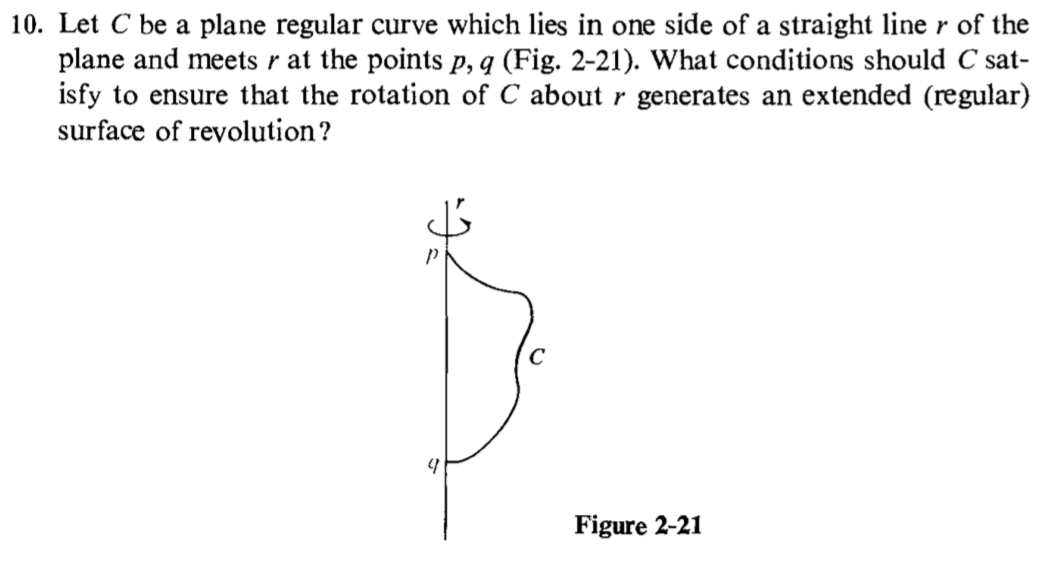
\includegraphics[scale=0.7]{Ca.png}
\end{problem}

\newpage
\begin{problem}
 b) Problem 9 on page 89, Section 2-4, Baby Do Carmo.
 
 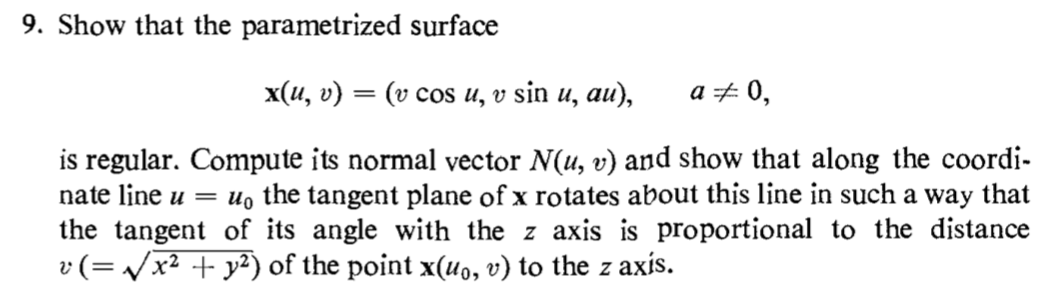
\includegraphics[scale=0.7]{Cb.png}
\end{problem}
\newpage
\begin{problem}
c) Problem 15 on page 90, Section 2-4, Baby Do Carmo.

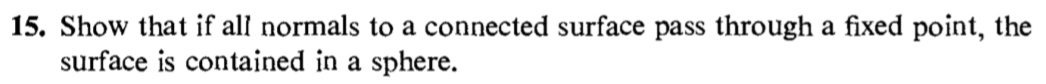
\includegraphics[scale=0.7]{Cc.png}
\end{problem}

\newpage
\begin{problem}
d) Problem 18 on page 90, Section 2-4, Baby Do Carmo.

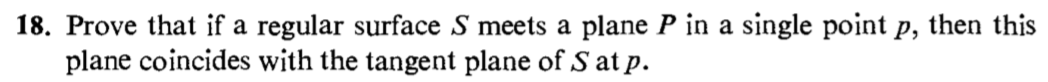
\includegraphics[scale=0.7]{Cd.png}
\end{problem}

\newpage
\begin{problem}
e) Problem 1 on page 99, Section 2-5, Baby Do Carmo.

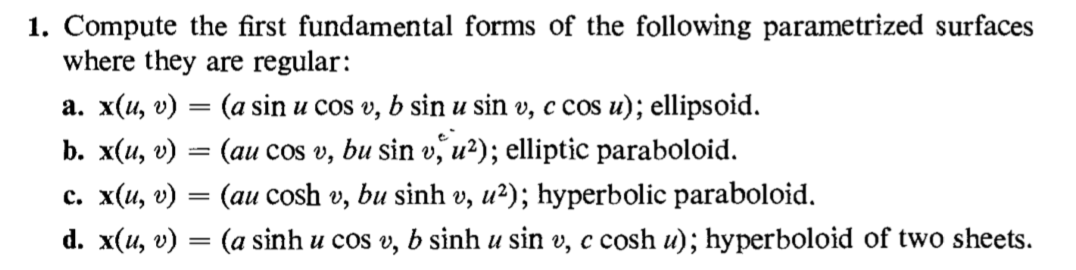
\includegraphics[scale=0.7]{Ce.png}
\end{problem}
\begin{solution}
We will find the $\textbf{x}_u, \textbf{x}_v$ for each problem. From there we
find $E=<\textbf{x}_u, \textbf{x}_u>, F - <\textbf{x}_u, \textbf{x}_v>,
G=<\textbf{u}_v, \textbf{u}_v>$. Then the first fundamental form is,
\begin{align*}
  I_p((u', v')) = E (u')^2 + 2Fu'v' + G(v')^2
\end{align*}
where $p$ is a point on the surface. \\
\begin{enumerate}[(a)]
\item $\textbf{x}_u = (a \cos u \cos v, b \cos u \sin v, -c \sin u),
  \textbf{x}_v = (-a \sin u \sin v, \sin u \cos v, 0)$.
\item $\textbf{x}_u = (a \cos v, b \sin v, 2u), \textbf{x}_v = (-au \sin v, bu
  \cos v, 0)$
\end{enumerate}
\end{solution}

\newpage
\begin{problem}
f) Problem 3 on page 99, Section 2-5, Baby Do Carmo.

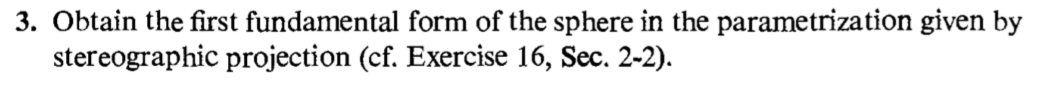
\includegraphics[scale=0.7]{Cf.png}
\end{problem}
The parameterization for the surface is,
\begin{align*}
  \pi^{-1}(u, v) = \begin{bmatrix}
    \frac{4u}{u^2 + v^2 + 4} \\
    \frac{4v}{u^2 + v^2 + 4} \\
    \frac{2(u^2 + v^2)}{u^2 + v^2 + 4}
    \end{bmatrix}
\end{align*}
Then,
\begin{align*}
  \boldsymbol{\pi^{-1}}_u = \begin{bmatrix}
    \frac{4}{u^2 + v^2 + 4} - \frac{4u}{(u^2 + v^2 + 4)^2} \cdot 2u \\
    -\frac{4v}{(u^2 + v^2 + 4)^2} \cdot 2u \\
    \frac{4u}{u^2 + v^2 + 4} - \frac{2(u^2 + v^2)}{(u^2 + v^2 + 4)^2} \cdot 2u
  \end{bmatrix} \\
  \boldsymbol{\pi^{-1}}_v = \begin{bmatrix}
    -\frac{4u}{(u^2 + v^2 + 4)^2} \cdot 2v \\
    \frac{4}{u^2 + v^2 + 4} - \frac{4v}{(u^2 + v^2 + 4)^2} \cdot 2v \\
    \frac{4v}{u^2 + v^2 + 4} - \frac{2(u^2 + v^2)}{(u^2 + v^2 + 4)^2} \cdot 2v
  \end{bmatrix}
\end{align*}
Then calcualate the first fundamental form as described in the last problem. 
\newpage
\begin{problem}
g) Problem 9 on page 100, Section 2-5, Baby Do Carmo.

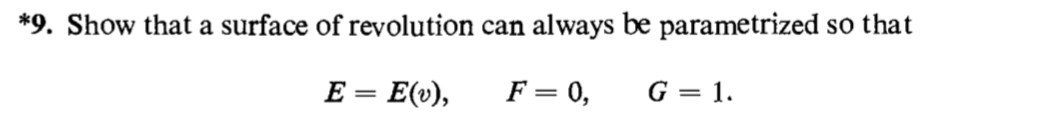
\includegraphics[scale=0.7]{Cg.png}
\end{problem}
%Consider a function $f: R \rightarrow R$ that we want to revolve around the x axis in
%order to obtain a surface of revolution. Then the parameterization for the
%surface would be,
%\begin{align*}
%  \mathbf{x}(u, v) = (f(u) \cos \frac{v}{f(u)}, f(u) \sin \frac{v}{f(u)}, u) 
%\end{align*}
%
%So,
%\begin{align*}
%  \textbf{x}_u = \begin{bmatrix}
%
%    f'(u) \cos \frac{v}{f(u)} - \sin (\frac{v}{f(u)}) \frac{v}{f(u)}f'(u) \\
%    1
%   \end{bmatrix}
%\end{align*}
%for $u \in [0, z_f], v \in [0, 2\pi]$. Then $E=<\textbf{x}_u, \textbf{x}_u> = E(u) $
\newpage
\textbf{D: Extra Credit Problems}

\begin{problem}
a) Let $T\subset R^3$ be a torus of revolution with center in 
$(0,0,0)\in R^3$ and let $A(x,y,z)=(-x,-y,-z)$.
Let $K$ be the quotient space of the torus $T$ by the equivalence 
relation $p\sim A(p)$.  Can you tell what surface $K$ is? 
\end{problem}

\newpage
\begin{problem}
b) Show that $K$ is a differentiable 2-dimensional manifold.
\end{problem}

\newpage
\begin{problem}
c) Show that $K$ is non orientable in two different ways.
\end{problem}

\end{document}

